\chapter{Технологический раздел}



\section{Выбор языка программирования}

Для реализации разработанного метода должен быть выбран язык, предоставляющий возможность создавать собственные менеджеры памяти. При этом он должен иметь встроенный сборщик мусора, что позволит провести сравнительный анализ разработанного метода с существующей реализацией в рамках одного языка при использовании разных менеджеров памяти. По этим причинам в качестве языка реализации был выбран Golang~\cite{golang}.

% В качестве языка реализации разработанного метода был выбран язык Golang~\cite{golang}, поскольку он предоставляет возможность разрабатывать собственные менеджеры памяти, при этом он уже имеет встроенный сборщик мусора, что позволяет провести сравнительный анализ разработанного метода с существующей реализацией в рамках одного языка при использовании разных менеджеров памяти.

%Выбор языка
%Необходимое условие 1: набирает популярность на бэке (серверное ПО), уже имеет заметный кусок рынка, относительно низкая стоимость разработки
%Необходимое условие 2: есть возможность разрабатывать собственные менеджеры памяти
%Необходимое условие 3: не запрещёна полностью ФСТЭК
%Достаточное условие: в языке уже есть автоматический менеджер памяти, который можно настраивать и с которым можно сравниться, находясь в рамках одного и того же языка при использовании разных менеджеров памяти
%Ответ: Golang
\clearpage
\section{Арены памяти}

В версии Golang 1.20 появилось экспериментальное решение для управления памятью, которое позволяет совместить безопасное выделение динамической памяти и уменьшение влияния среды выполнения языка, включающей интегрированный менеджер памяти, на производительность приложения.

% С точки зрения распределения памяти работа с ареной похожа на выделение одной области памяти (который может увеличиваться в размере) и при освобождении арены все выделенные в ней объекты становятся недоступными.

Пакет arena предоставляет альтернативную возможность выделения памяти в программах на языке Golang. Освобождать такую память необходимо вручную, причем безопасно и всю одновременно. Цель этой функциональности --- повышение эффективности программ: ручное освобождение памяти откладывает следующий цикл сборки мусора. В свою очередь, снижение частоты циклов означает уменьшение накладных расходов на сборку мусора. \cite{golang_arena_cource}

Большая часть описанной функциональности рассматриваемого пакета реализована в типе Arena, который является абстракцией относительно большого объёма памяти, выделенного в куче. Наиболее эффективное использование Arena достигается при хранении в них некоторого множества объектов программы, занимающих около 1 Мб памяти. \cite{golang_arena_cource} \cite{golang_arena_proposal}

Стоит заметить, что при использовании этой ограниченной формы ручного выделения памяти возможны ошибки типа <<use-after-free>> (использование после освобождения). Пакет Arena ограничивает влияние этих ошибок, предотвращая повторное использование освобождённых областей памяти до тех пор, пока сборщик мусора не сможет убедиться в том, что это безопасно. Как правило, ошибка <<use-after-free>> приводит к сбою и получению сообщения об ошибке, но пакет Arena оставляет за собой право не вызывать сбой программы при использовании освобождённой памяти. Это означает, что реализация данного пакета допускает выделение памяти так, как это обычно делает среда выполнения, оставляя за собой право иногда делать это для некоторых объектов программы.~\cite{golang_arena_cource}

Повышение производительности программы, использующей выделение памяти на аренах, можно ожидать в тех случаях, когда приложение интенсивно выделяет память (например, при работе с ссылочными структурами данных, такими как двоичные деревья), но при этом предполагается, что выделенные структуры данных являются относительно долгоживущими и существуют до момента освобождения всей арены целиком (сборщик мусора для арены не применяется и выделенные на ней объекты не освобождаются автоматически).

Стоит отметить, что если размер объекта превышает 25\% размера пустой арены, то он будет выделен за пределами арены и его жизненный цикл будет контролироваться встроенным сборщиком мусора. Поэтому с точки зрения разрабатываемого метода такие объекты считаются \textbf{неконтролируемыми}, при этом их ссылки могут быть проанализированы и факт их финализации сборщиком мусора может быть определён.

\section{Компоненты программного обеспечения}

Разработанный метод распределения памяти был реализован в виде подключаемой библиотеки, состоящей из следующих компонентов.

\begin{enumerate}[label*=\arabic*.]
	\item \textbf{Арена} (arena), предназначенная для выделения и хранения объектов программы. Стоит отметить, что арены из пакета arena языка Golang имеют неявные ограничения по размеру и количеству выделяемых объектов: если размер объекта превышает 25\% размера арены или размер свободной памяти в ней, то он выделяется за пределами арены, что может свести к нулю выигрыш во времени выделения памяти по сравнению со стандартными средствами языка Golang. \cite{golang_arena_limits} По этой причине был реализован обёрточный класс limited\_arena, реализующий описанное ограничение явно. 
	\item \textbf{Дескриптор объекта} (metadata), предназначенный для сохранения данных о выделяемых объектах (см. п. \ref{descriptor}).
	\item \textbf{Поколение} (generation), предназначенное для хранения дескрипторов выделенных объектов и поддерживающее операции сборки мусора и перемещения объектов между поколениями. Поколение не хранит отдельные объекты напрямую, а использует для этого арены памяти фиксированного размера.
	\item \textbf{Память} (memory), являющаяся абстракцией, хранящей все поколения и предназначенной для обработки внешних запросов на выделение памяти в куче.
	\item \textbf{Гипервизор} (hypervisor), отвечающий за выполнение сборки мусора и перераспределение объектов между поколениями по итогам сбора. Именно гипервизор определяет момент, когда необходимо провести сборку мусора.
	\item \textbf{Разметчик} (mark worker), предназначенный для разметки объектов, выделенных менеджером памяти. Он работает в одном потоке программы, поэтому поколение для проведения параллельной разметки запускает несколько разметчиков в отдельных потоках программы и ожидает завершения их работы.
\end{enumerate}

Структуры, описывающие основные компоненты реализованной библиотеки, представлены на рисунке \ref{fig:struct} в виде диаграммы классов.

\begin{figure}[H]
	\centering
	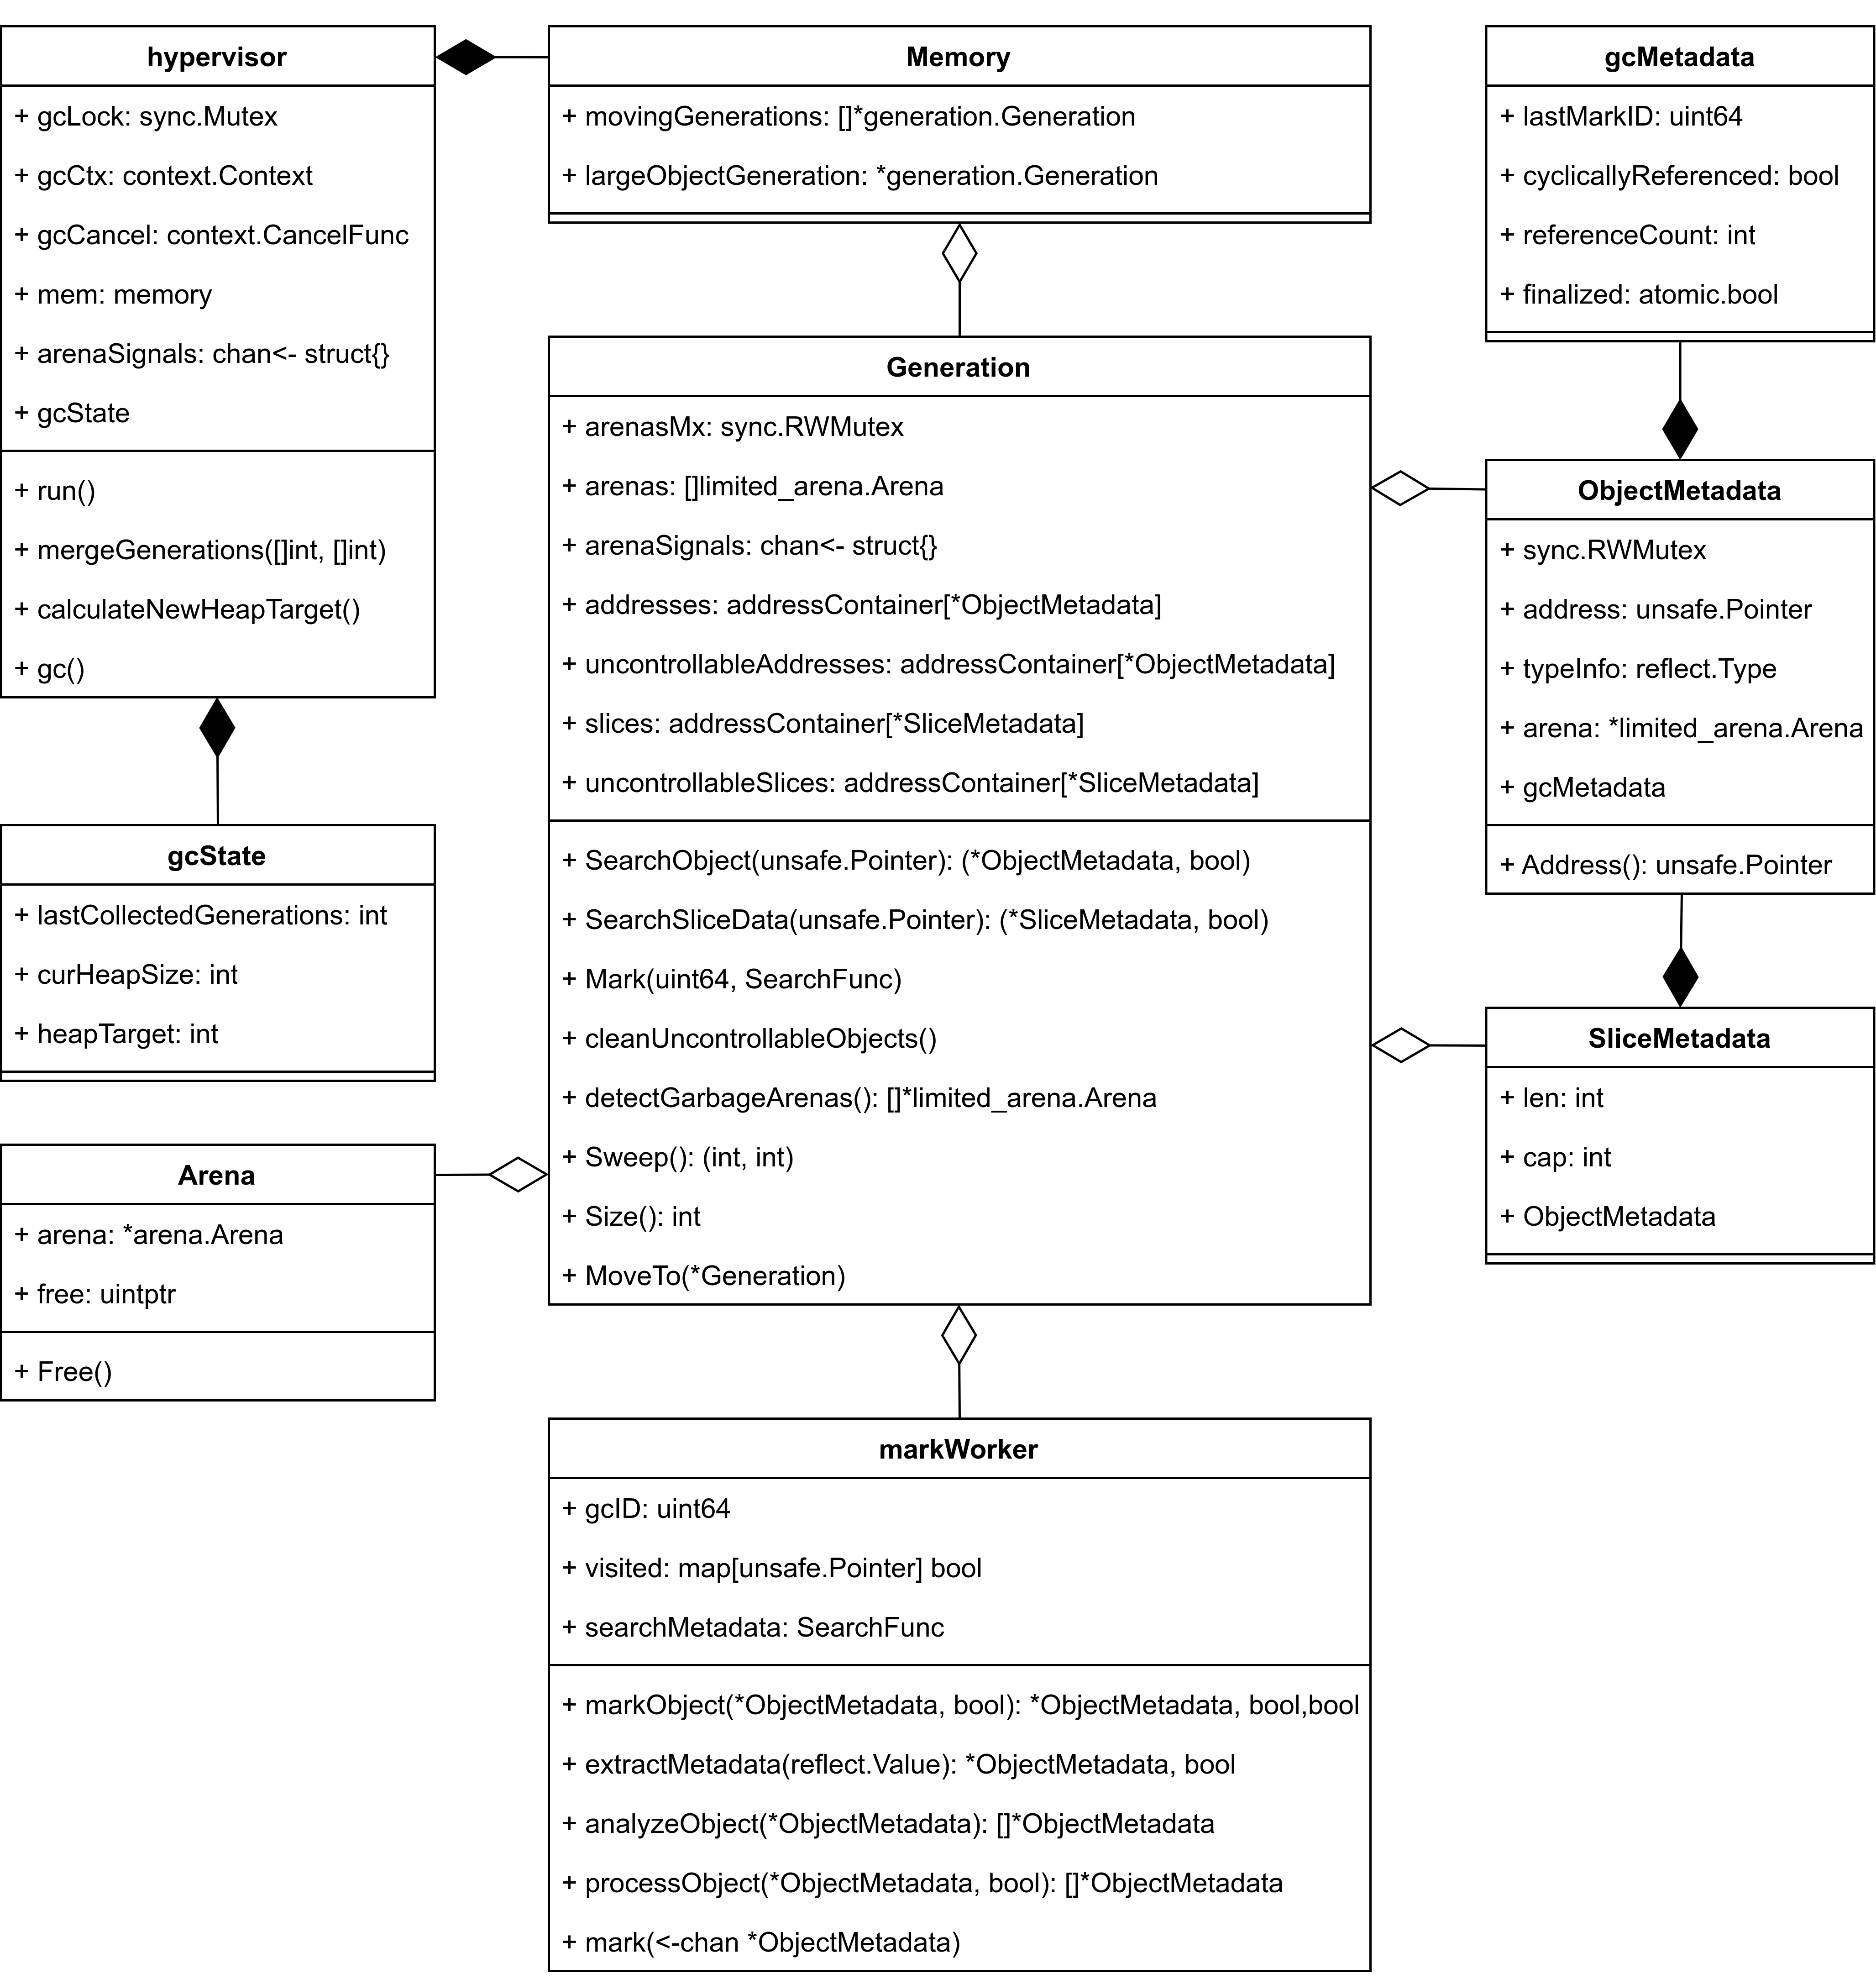
\includegraphics[width=\textwidth]{assets/uml.png}
	\caption{Диаграмма классов разработанной библиотеки}
	\label{fig:struct}
\end{figure}

%\begin{lstlisting}[
%	caption={Основоные компоненты библиотеки},
%	label=lst:struct]
%type Arena struct {
%	arena *arena.Arena
%	free  uintptr
%}
%
%type ObjectMetadata struct {
%	sync.RWMutex
%	address  unsafe.Pointer
%	typeInfo reflect.Type
%	gcMetadata
%}
%
%type SliceMetadata struct {
%	ObjectMetadata
%	len int
%	cap int
%}
%
%type Generation struct {
%	arenasMx                sync.RWMutex
%	arenas                  []limited_arena.Arena
%	arenaSignals            chan<- struct{}
%	addresses               addressContainer[*ObjectMetadata]
%	uncontrollableAddresses addressContainer[*ObjectMetadata]
%	slices                  addressContainer[*SliceMetadata]
%	uncontrollableSlices    addressContainer[*SliceMetadata]
%}
%
%type memory struct {
%	movingGenerations     []*generation.Generation
%	largeObjectGeneration *generation.Generation
%}
%
%type gcState struct {
%	lastCollectedGenerations int
%	curHeapSize              int
%	heapTarget               int
%}
%
%type hypervisor struct {
%	gcLock       sync.Mutex
%	gcCtx        context.Context
%	gcCancel     context.CancelFunc
%	mem          memory
%	arenaSignals <-chan struct{}
%	gcState
%}
%\end{lstlisting}

%Публичные функции и интерфейсы разработанной библиотеки представлены на листинге \ref{lst:public}.
%
%\begin{lstlisting}[
%	caption={Публичные функции и интерфейсы разработанной библиотеки},
%	label=lst:public]
%type Getter[T any] interface {
%	Get() *T
%}
%
%type SliceGetter[T any] interface {
%	Get() []T
%}
%
%type getter[T any] struct {
%	metadata *generation.ObjectMetadata
%	get      func() *T
%}
%
%func (g getter[T]) Get() *T {
%	return g.get()
%}
%
%type sliceGetter[T any] struct {
%	metadata *generation.ObjectMetadata
%	get      func() []T
%}
%
%func (g sliceGetter[T]) Get() []T {
%	return g.get()
%}
%
%func New[T any]() Getter[T] {
%	metadata, get, finalize := allocateObject[T](mainHypervisor.mem)
%	g := getter[T]{
%		metadata: metadata,
%		get:      get,
%	}
%	runtime.SetFinalizer(&g, func(_ *getter[T]) { finalize() })
%	
%	return g
%}
%
%func MakeSlice[T any](len, cap int) SliceGetter[T] {
%	metadata, get, finalize := allocateSlice[T](
%		mainHypervisor.mem, len, cap,
%	)
%	g := sliceGetter[T]{
%		metadata: metadata,
%		get:      get,
%	}
%	runtime.SetFinalizer(&g, func(_ *getter[T]) { finalize() })
%	
%	return g
%}
%
%func Append[T any](getter SliceGetter[T], elems ...T) {
%	appendSlice(mainHypervisor.mem, getter.Get(), elems...)
%}
%
%func Clone[T any](getter Getter[T]) T {
%	return arena.Clone[T](*getter.Get())
%}
%
%func CloneSlice[S ~[]E, E any](getter SliceGetter[E]) S {
%	return arena.Clone[S](getter.Get())
%}
%
%func GC() {
%	if mainHypervisor.gcLock.TryLock() {
%		mainHypervisor.gc()
%		
%		ctx, cancel := context.WithCancel(context.Background())
%		mainHypervisor.gcCancel()
%		mainHypervisor.gcCancel = cancel
%		
%		Debugger.numCC.Add(1)
%		Debugger.lastCC.Store(time.Now().Unix())
%		
%		mainHypervisor.gcLock.Unlock()
%		
%		mainHypervisor.gcCtx = ctx
%	} else {
%		<-mainHypervisor.gcCtx.Done()
%	}
%}
%\end{lstlisting}



\subsection{Выделение памяти в куче}

Функции выделения памяти в куче, определённые для объекта memory, представлены на листинге \ref{lst:alloc}. Все новые объекты выделяются в молодом поколении. Если размер объекта превышает 85000 байт, то он выделяется в специальном поколении больших объектов, чтобы реже всего подвергаться анализу.

\begin{lstlisting}[
caption={Функции выделения памяти},
label=lst:alloc]
const objectSizeThreshold = 85_000

func allocateObject[T any](mem memory) (
	m *generation.ObjectMetadata, get func() *T, finalize func(),
) {
	size := unsafe.Sizeof(*new(T)) // no allocation
	if size > objectSizeThreshold {
		return generation.AllocateObject[T](mem.largeObjectGeneration)
	}
	return generation.AllocateObject[T](mem.movingGenerations[0])
}

func allocateSlice[T any](mem memory, len, cap int) (
	m *generation.ObjectMetadata, get func() []T, finalize func(),
) {
	size := unsafe.Sizeof(*new(T)) * uintptr(cap) // no allocation
	if size > objectSizeThreshold {
		m, get, finalize = generation.AllocateSlice[T](
			mem.largeObjectGeneration, len, cap,
		)
	} else {
		m, get, finalize = generation.AllocateSlice[T](
			mem.movingGenerations[0], len, cap,
		)
	}
	return
}
\end{lstlisting}



\subsection{Выделение памяти в поколении}

Функции выделения памяти в поколении объектов представлены на листинге \ref{lst:gen-alloc}. Аллокация обычных объектов и срезов выполняется по одному алгоритму, однако требует выполнения различных операций по формированию возвращаемых значений, поэтому реализована в отдельных функциях. Функция добавления элементов в срез необходима для обновления его адреса в случае перевыделения.

\begin{lstlisting}[
caption={Функции выделения памяти в поколении объектов},
label=lst:gen-alloc]
type holder[T any] interface {
	*T | []T
}

type allocateFunc[H holder[T], T any] func(*limited_arena.Arena) (H, bool)

type allocatedObject[T any, H holder[T]] struct {
	container    H
	controllable bool
	arena        *limited_arena.Arena
}

func allocate[T any, H holder[T]](
	gen *Generation, allocateObject allocateFunc[H, T],
) allocatedObject[T, H] {
	gen.arenasMx.Lock()
	var object allocatedObject[T, H]
	for _, arena := range gen.arenas {
		object.container, object.controllable = allocateObject(&arena)
		if object.container != nil {
			object.arena = &arena
			break
		}
	}
	if object.container == nil {
		arena := limited_arena.NewLimitedArena()
		gen.arenaSignals <- struct{}{}
		object.container, object.controllable = allocateObject(&arena)
		object.arena = &arena
		gen.arenas = append(gen.arenas, arena)
	}
	gen.arenasMx.Unlock()
	
	return object
}

func AllocateObject[T any](gen *Generation) (
	m *ObjectMetadata, get func() *T, finalize func(),
) {
	object := allocate[T](gen, limited_arena.New[T])
	
	metadata := ObjectMetadata{
		address:  unsafe.Pointer(object.container),
		typeInfo: reflect.TypeOf(*object.container),
		arena:    object.arena,
	}
	
	if !object.controllable {
		gen.uncontrollableAddresses.Add(&metadata)
	} else {
		gen.addresses.Add(&metadata)
	}
	
	get = func() *T {
		metadata.RLock()
		res := (*T)(metadata.address)
		metadata.RUnlock()
		return res
	}
	finalize = func() {
		finalized := metadata.finalized.Swap(true)
	}
	
	return &metadata, get, finalize
}

func makeSliceFromPtr[T any](ptr unsafe.Pointer, len, cap int) []T {
	return unsafe.Slice((*T)(ptr), cap)[:len]
}

func AllocateSlice[T any](gen *Generation, len, cap int) (
	m *ObjectMetadata, get func() []T, finalize func(),
) {
	object := allocate[T](
		gen, func(arena *limited_arena.Arena) ([]T, bool) {
			return limited_arena.MakeSlice[T](arena, len, cap)
		},
	)
	
	metadata := SliceMetadata{
		ObjectMetadata: ObjectMetadata{
			address:  unsafe.Pointer(&object.container[0]),
			typeInfo: reflect.TypeOf(object.container),
			arena:    object.arena,
		},
		len: len,
		cap: cap,
	}
	
	if !object.controllable {
		gen.uncontrollableSlices.Add(&metadata)
	} else {
		gen.slices.Add(&metadata)
	}
	
	get = func() []T {
		metadata.RLock()
		res := makeSliceFromPtr[T](
			metadata.address, metadata.len, metadata.cap,
		)
		metadata.RUnlock()
		return res
	}
	finalize = func() {
		finalized := metadata.finalized.Swap(true)
	}
	
	return &metadata.ObjectMetadata, get, finalize
}
\end{lstlisting}



\subsection{Сбор мусора в поколении}

Сбор мусора проводится для каждого поколения отдельно и состоит из разметки, очистки и перераспределения данных между поколениями. Первые два этапа реализует поколение, а третий --- гипервизор, принимающий решение о том, стоит ли переносить объекты из одного поколения в другое после очередного цикла сбора мусора. Также именно гипервизор устанавливает целевой размер кучи, по достижении которого будет осуществлён следующий цикл сбора мусора.

\subsubsection{Разметка}

Реализация алгоритма разметки объектов поколения представлена на листинге \ref{lst:gen-mark}. Для выполнения параллельной разметки запускается несколько разметчиков в отдельных потоках программы. Ограничение количества запущенных разметчиков по умолчанию равно половине от количества процессорных ядер, доступных программе.

\begin{lstlisting}[
caption={Реализация алгоритма разметки объектов поколения},
label=lst:gen-mark]
var gcMarkConcurrency = (runtime.NumCPU() + 1) / 2

type SearchFunc func(addr unsafe.Pointer) (
	metadata *ObjectMetadata, exist bool,
)

func (gen *Generation) Mark(gcID uint64, searchMetadata SearchFunc) {
	search := func(addr unsafe.Pointer) (
		metadata *ObjectMetadata, exist bool,
	) {
		metadata, exist = gen.SearchObject(addr)
		if !exist {
			metadata, exist = searchMetadata(addr)
		}
		return
	}
	
	objects := make(chan *ObjectMetadata)
	wg := sync.WaitGroup{}
	for range gcMarkConcurrency {
		mw := markWorker{
			gcID:           gcID,
			visited:        make(map[unsafe.Pointer]bool),
			searchMetadata: search,
		}
		wg.Add(1)
		go func() {
			mw.mark(objects)
			wg.Done()
		}()
	}
	
	gen.addresses.Map(func(metadata *ObjectMetadata) {
		metadata.cyclicallyReferenced = false
		metadata.referenceCount--
		objects <- metadata
	})
	
	gen.slices.Map(func(metadata *SliceMetadata) {
		metadata.cyclicallyReferenced = false
		metadata.referenceCount--
		objects <- &metadata.ObjectMetadata
	})
	
	close(objects)
	wg.Wait()
}
\end{lstlisting}

Реализация алгоритма обработки одного объекта представлена на листинге \ref{lst:gen-process}. При рекурсивном обходе графа объектов разметчик обнаруживает циклические ссылки, исключая ссылки объекта на самого себя.

\begin{lstlisting}[
	caption={Реализация алгоритма обработки одного объекта},
	label=lst:gen-process]
func (mw markWorker) processObject(
	object *ObjectMetadata, visited bool,
) (rcSrcs []*ObjectMetadata) {
	object.Lock()
	rcSrc, skip, visited := mw.markObject(object, !visited)
	if !skip {
		nextObjects := mw.analyzeObject(object)
		object.Unlock()
		for _, nextObject := range nextObjects {
			if nextObject == object {
				continue
			}
			rcSrcs = append(rcSrcs, 
				mw.processObject(nextObject, visited)...,
			)
			delete(mw.visited, nextObject.address)
			if len(rcSrcs) != 0 {
				object.cyclicallyReferenced = true
				rcSrcs = slices.DeleteFunc(
					rcSrcs, func(metadata *ObjectMetadata) bool {
						return metadata == object
					}
				)
			}
		}
	} else {
		object.Unlock()
		rcSrcs = append(rcSrcs, rcSrc)
	}
	
	return
}
\end{lstlisting}

Реализация алгоритма разметки одного объекта представлена на листинге \ref{lst:gen-mark-one}. Разметка объекта включает в себя подсчёт ссылок на объект, определение факта участия рассматриваемого объекта в цикле ссылок и принятие решения о дальнейшей обработке его ссылок на другие объекты программы.

\begin{lstlisting}[
caption={Реализация алгоритма разметки объекта},
label=lst:gen-mark-one]
func (mw markWorker) markObject(object *ObjectMetadata, incRefCount bool) (
	rcSrc *ObjectMetadata, skip, visited bool,
) {
	if object.finalized.Load() {
		return nil, true, false
	}
	
	if incRefCount {
		object.referenceCount++
	}
	
	if object.lastMarkID == mw.gcID {
		if mw.visited[object.address] {
			object.cyclicallyReferenced = true
			return object, true, true
		} else {
			mw.visited[object.address] = true
			return nil, false, true
		}
	} else {
		object.lastMarkID = mw.gcID
		mw.visited[object.address] = true
		return nil, false, false
	}
}
\end{lstlisting}

Реализация алгоритма анализа ссылок объекта представлена на листинге \ref{lst:gen-analyze}. Извлечение ссылок объекта производится с помощью библиотеки reflect. После извлечения ссылок на другие объекты производится поиск их дескрипторов в множестве доступных для разметки адресов, которое может изменяться между циклами сборки мусора вместе с количеством поколений, анализируемых в текущем цикле сборки. Чем шире область поиска, тем больше ссылок между объектами можно обнаружить и тем выше вероятность обнаружения цикла ссылок меду объектами программы.

\begin{lstlisting}[
caption={Реализация алгоритма анализа ссылок объекта},
label=lst:gen-analyze]
func (mw markWorker) analyzeObject(metadata *ObjectMetadata) (
	nextObjects []*ObjectMetadata,
) {
	object := reflect.NewAt(metadata.typeInfo, metadata.address).Elem()
	nestedObjects := extractNestedObjects(object)
	for _, nestedObject := range nestedObjects {
		nestedMetadata, exist := mw.extractMetadata(nestedObject)
		if exist {
			nextObjects = append(nextObjects, nestedMetadata)
		}
	}
	
	return
}
\end{lstlisting}



\subsubsection{Очистка}

Реализация алгоритма очистки поколения от мусорных объектов представлена на листинге \ref{lst:gen-sweep}. Очистка производится в одном потоке программы и состоит в удалении не отдельных объектов, а арен, состоящих только из мусорных объектов.

\begin{lstlisting}[
caption={Реализация алгоритма очистки поколения от мусорных объектов},
label=lst:gen-sweep]
func (gen *Generation) Sweep() (int, int) {
	gen.arenasMx.Lock()
	
	sizeBefore := len(gen.arenas)
	
	garbageArenas := gen.detectGarbageArenas()
	if len(garbageArenas) == 0 {
		return sizeBefore, sizeBefore
	}
	
	for offset, arena := range garbageArenas {
		index := slices.Index(gen.arenas, *arena)
		tailIndex := len(gen.arenas) - offset - 1
		gen.arenas[index] = gen.arenas[tailIndex]
		gen.arenas[tailIndex].Free()
		gen.arenas[tailIndex] = limited_arena.Arena{}
	}
	
	gen.arenas = gen.arenas[:len(gen.arenas)-len(garbageArenas)]
	
	gen.arenasMx.Unlock()
	
	return sizeBefore, sizeBefore - len(garbageArenas)
}
\end{lstlisting}

Реализация алгоритма обнаружения мусорных арен представлена на листинге \ref{lst:gen-detect}. Очистка производится в одном потоке программы и состоит в удалении не отдельных объектов, а арен, состоящих только из мусорных объектов.

\begin{lstlisting}[
caption={Реализация алгоритма обнаружения мусорных арен},
label=lst:gen-detect]
func (gen *Generation) cleanUncontrollableObjects() {
	garbageObjects := make([]unsafe.Pointer, 0)
	gen.uncontrollableAddresses.Map(func(object *ObjectMetadata) {
		if object.finalized.Load() {
			garbageObjects = append(garbageObjects, object.address)
		}
	})
	gen.uncontrollableAddresses.Delete(garbageObjects)
	
	garbageSlices := make([]unsafe.Pointer, 0)
	gen.uncontrollableSlices.Map(func(slice *SliceMetadata) {
		if slice.finalized.Load() {
			garbageSlices = append(garbageSlices, slice.address)
		}
	})
	gen.uncontrollableSlices.Delete(garbageSlices)
}

func isGarbage(object *ObjectMetadata) bool {
	return (object.cyclicallyReferenced && object.referenceCount <= 1) || 
		object.finalized.Load()
}

func (gen *Generation) detectGarbageArenas() []*limited_arena.Arena {
	arenaObjectsCount := make(map[*limited_arena.Arena]int, len(gen.arenas))
	garbageObjectsCount := make(
		map[*limited_arena.Arena]int, len(gen.arenas),
	)
	
	garbageAddresses := make([]unsafe.Pointer, 0)
	garbageSlices := make([]unsafe.Pointer, 0)
	
	gen.addresses.Map(func(object *ObjectMetadata) {
		arenaObjectsCount[object.arena]++
		if isGarbage(object) {
			garbageObjectsCount[object.arena]++
			garbageAddresses = append(garbageAddresses, object.address)
		}
	})
	
	gen.slices.Map(func(object *SliceMetadata) {
		arenaObjectsCount[object.arena]++
		if isGarbage(&object.ObjectMetadata) {
			garbageObjectsCount[object.arena]++
			garbageSlices = append(garbageSlices, object.address)
		}
	})
	
	garbageArenas := make([]*limited_arena.Arena, 0)
	for arena, count := range arenaObjectsCount {
		if garbageObjectsCount[arena] == count && count != 0 {
			garbageArenas = append(garbageArenas, arena)
		}
	}
	
	gen.addresses.Delete(garbageAddresses)
	gen.slices.Delete(garbageSlices)
	gen.cleanUncontrollableObjects()
	
	return garbageArenas
}
\end{lstlisting}



\subsubsection{Перераспределение объектов между поколениями}

После завершения очистки мусорных арен в каждом поколении гипервизор на основании результатов сбора принимает решение о продвижении объектов по поколениям. Перемещение каждого объекта происходит до тех пор, пока он не окажется в последнем (<<постоянном>>) поколении. Также стоит отметить, что перемещению не подвергаются объекты, выделенные в поколении <<больших>> объектов (см. п. \ref{concepts}).

\begin{lstlisting}[
caption={Реализация алгоритма перераспределения объектов между поколениями},
label=lst:gen-move]
const generationMovementThreshold = 0.9

func (h *hypervisor) mergeGenerations(sizesBefore, sizesAfter []int) {
	for i := len(sizesBefore) - 3; i >= 0; i-- {
		if float64(sizesAfter[i])/float64(sizesBefore[i]) <=
			generationMovementThreshold {
			h.mem.movingGenerations[i].MoveTo(h.mem.movingGenerations[i+1])
		}
		if sizesBefore[i] != sizesAfter[i] {
			Debugger.arenasFreed.Add(int64(sizesBefore[i] - sizesAfter[i]))
		}
	}
}
\end{lstlisting}


\section{Оценка трудоёмкости алгоритмов}

Для определения гарантии времени исполнения необходимо оценить трудоёмкость выполнения мутатором выделения памяти и обращения к выделенным объектам. Трудоёмкость реализаций алгоритмов будет оцениваться только для худшего случая, так как именно его рассмотрение поможет определить гарантию времени выполнения реализованного метода.

\subsection{Модель вычислений}

Для последующего вычисления трудоемкости необходимо ввести модель вычислений.

\begin{enumerate}
	\item Операции из списка \ref{for:opers_1} имеют трудоемкость 1.
	\begin{equation}
		\label{for:opers_1}
		+, -, =, +=, -=, ==, !=, <, >, <=, >=, [], ++, {-}-, \&\&, ||, !
	\end{equation}

	\item Операции индексации, разыменования указателя, получения адреса, определения размера типа данных, блокировки и разблокировки мьютекса, создания пустого среза и определения его длины, удаления элемента из среза и отправки данных в канал имеют трудоёмкость 1.
	
	\item Трудоёмкость условного оператора вида <<if условие then A else B>> определяется по формуле \ref{for:if}.
	\begin{equation}
		\label{for:if}
		f_{if} = f_{\text{условие}} +
		\begin{cases}
			f_A, & \text{если условие выполняется,}\\
			f_B, & \text{иначе.}
		\end{cases}
	\end{equation}

	\item Трудоёмкость цикла for, предполагающего выполнение $N$ итераций, определяется по формуле \ref{for:for}.
	\begin{equation}
		\label{for:for}
		f_{for} = f_{\text{инициализация}} + f_{\text{сравнение}} + N(f_{\text{тело}} + f_{\text{инкремент}} + f_{\text{сравнение}})
	\end{equation}
	
	\item Трудоёмкость цикла for range по коллекции из $N$ элементов определяется по формуле \ref{for:range}.
	\begin{equation}
		\label{for:range}
		f_{for} = f_{\text{инициализация}} + N(f_{\text{тела}} + f_{\text{присваивание}})
	\end{equation}
	
	\item Трудоёмкость вызова функции и преобразования типа данных переменной равна 0.
	
	\item Операция добавления элемента в срез имеет трудоёмкость 7.
	
	\item Трудоёмкость получения ссылок объекта, создания экземпляра reflect.Value по указателю на объект, выделения памяти в арене, создания и освобождения арены, а также создания горутины равна 25.
\end{enumerate}


\subsection{Трудоёмкость реализации алгоритма выделения памяти}

Худшим случаем для оценки трудоёмкости реализации алгоритма выделения памяти является тот, в котором алгоритм начинает выполняться одновременно с очисткой поколения, при этом все его объекты должны являться мусорными. Так как данные процедуры не могут выполняться параллельно, для выполнения выделения памяти в поколении необходимо дождаться завершения его очистки от мусорных объектов.

В худшем случае трудоёмкость реализации алгоритма выделения памяти без учёта очистки определяется по формуле \ref{for:allocateObject}.
\begin{equation}
	\label{for:allocateObject}
	f_{allocateObject}^{\wedge} = 3 + f_{AllocateObject}^{\wedge} = 21 + f_{allocate}^{\wedge} = 21 + 71 = 92
\end{equation}
% AllocateObject = 1 + allocate + 5 + 1 + 1 + 7 + 1 + 1 + 1 = allocate + 18 = 89
% allocate = 2 + 1 + 25 + 1 + 2 + 2 + 25 + 2 + 7 + 2 + 2 = 71

В худшем случае трудоёмкость реализации алгоритма очистки поколения от мусорных объектов определяется по формуле \ref{for:Sweep}.
\begin{equation}
	\label{for:Sweep}
	\begin{array}{l}
		f_{detectGarbageArenas}^{\wedge} = 13 + 24c + 14a + o + 12*u = 13 + 25c + 14a +\\+ 13u\\
		f_{Sweep}^{\wedge} = 19 + 43a + a^2 + f_{detectGarbageArenas}^{\wedge} = 32 + 57a + 25c + 13u +\\+ a^2,
	\end{array}
\end{equation}
% sweep = 4 + 1 + dga + 2 + for + 8 + 2 = 17 + dga + for
% for = 2 + A_GA * (A_GA + 3 + 5 + 5 + 2 + 25 + 3) = 2 + A_GA^2 + 43*A_GA
% sweep = 17 + 2 + A_GA^2 + 43*A_GA + 13 + 24*OB_GOB + 14*A_GA + AGOB + 12*UO_GUO = 32 + 57*A_GA + 24*OB_GOB + AGOB + 12*UO_GUO + A_GA^2
где $a$ --- число арен в поколении, $с$ --- число контролируемых объектов, $u$ --- число неконтролируемых объектов, $o = c + u$ --- общее число объектов в поколении.

Таким образом, в худшем случае трудоёмкость реализации алгоритма выделения памяти определяется по формуле \ref{for:alloc-total}.

\begin{equation}
	\label{for:alloc-total}
	f_{allocation}^{\wedge} = f_{allocateObject}^{\wedge} + f_{Sweep}^{\wedge} = 124 + 57a + 25c + 13u + a^2
\end{equation}
% dga = 1 + 1 + 1 + 1 + for1 + for2 + 1 + for3 + 2 + GO*1 + 1 + for4 + 1 + for5
% ig = 6
% for1 = for2 = 1 + OB_GOB*(1 + 3 + 2 + 6 + 3 + 1 + 7 + 1) = 1 + 24*OB_GOB
% for3 = 2 + A_GA*(2 + 4 + 7 + 1) = 2 + 14*A_GA
% for4 = for5 = 1 + UO_GUO*(1 + 2 + 7 + 2) = 1 + 12*UO_GUO
% dga = 4 + 2 + 24*OB_GOB + 1 + 2 + 14*A_GA + 2 + AGOB*1 + 2 + 12*UO_GUO = 13 + 24*OB_GOB + 14*A_GA + AGOB + 12*UO_GUO



\subsection{Трудоёмкость реализации алгоритма обращения к объекту}

Худшим случаем для оценки трудоёмкости реализации алгоритма обращения к объекту может является тот, в котором алгоритм начинает выполняться одновременно с разметкой объекта. Так как данные процедуры не могут выполняться параллельно, для выполнения обращения к объекту необходимо дождаться завершения его разметки.

В худшем случае трудоёмкость реализации алгоритма обращения к объекту без учёта разметки равна 4.

В худшем случае трудоёмкость реализации алгоритма обработки объекта разметчиком определяется по формуле \ref{for:processObject}.
\begin{equation}
	\label{for:processObject}
	\begin{array}{l}
	f_{markObject}^{\wedge} = 11\\
	f_{analyzeObject}^{\wedge} = 55 + 13r + 2or\\
	f_{processObject}^{\wedge} = 9 + f_{markObject}^{\wedge} + f_{analyzeObject}^{\wedge} = 75 + 13r + 2or,
	\end{array}
\end{equation}
% processObject = 1 + 3 + 1 + mark + 2 + 1 + analyze + 1 = 9 + mark + analyze = 75 + 13*R + 2*O*R
% mark = 4 + 2 + 2 + 3 = 11
% analyze = 1 + 2 + 25 + 1 + 25 + 1 + R*(1 + 2 + 1 + O*(1 + 1) + 1 + 1 + 7) = 55 + 13*R + 2*O*R
где $r$ --- число ссылок рассматриваемого объекта на другие объекты, $o$ --- число объектов, участвующих в текущем цикле сборки.



\section{Руководство пользователя}

Библиотека, реализующая разработанный метод, может использоваться в программах на языке Golang версии 1.22.0 и выше. Для подключения библиотеки в проект необходимо установить её с помощью команды \ref{lst:cmd}.

\begin{lstlisting}[
	caption={Команда установки библиотеки},
	label=lst:cmd]
go get github.com/Inspirate789/alloc
\end{lstlisting}

Далее её можно использовать в проекте, не изменяя процесс сборки приложений. Примеры эквивалентных с точки зрения пользователя программ, использующих встроенные средства языка Golang и реализованную библиотеку, представлены на листингах \ref{lst:example-stdlib} и \ref{lst:example-alloc} соответственно.

\begin{lstlisting}[
caption={Программа, использующая встроенные средства языка Golang},
label=lst:example-stdlib]
package main

func main() {
	object := new(int)
	println(*object) // 0
	*object = 7
	println(*object) // 7
}
\end{lstlisting}

\begin{lstlisting}[
caption={Программа, использующая реализованную бибилотеку},
label=lst:example-alloc]
package main

import "github.com/Inspirate789/alloc"

func main() {
	object := alloc.New[int]()
	println(*object.Get()) // 0
	*object.Get() = 7
	println(*object.Get()) // 7
}
\end{lstlisting}

Стоит отметить, что для корректной работы сборщика мусора разработанного менеджера памяти не следует при работе с выделенными объектами игнорировать их геттеры, являющиеся барьерами чтения и записи. Так, программа, представленная на листинге \ref{lst:example-bad-alloc}, аналогична \ref{lst:example-stdlib} и \ref{lst:example-alloc} с точки зрения пользователя, однако может привести к гонкам данных при разметке объектов.

\begin{lstlisting}[
	caption={Программа, использующая реализованную бибилотеку},
	label=lst:example-bad-alloc]
	package main
	
	import "github.com/Inspirate789/alloc"
	
	func main() {
		object := alloc.New[int]().Get()
		println(*object)
		*object = 7
		println(*object)
	}
\end{lstlisting}



\section*{Выводы из технологического раздела}

В данном разделе было приведено обоснование выбора языка программирования для реализации разработанного метода. Было программное обеспечение, реализующее предложенный метод и были изложены его особенности.

Также была дана теоретическая оценка трудоёмкости выполнения вызовов реализации метода, а именно выделения памяти и обращения к выделенным объектам. В худшем случае трудоёмкость выделения памяти линейно зависит от числа объектов в самом <<молодом>> поколении и квадратично от числа арен в нём, при этом трудоёмкость обращения к объекту линейно зависит от числа ссылок в объекте и общего числа объектов, анализируемых сборщиком. Благодаря использованию модели поколений, сборщик мусора анализирует не все объекты, а только некоторую их часть. Таким образом удалось устранить зависимость накладных расходов мутатора от общего числа объектов во всей куче. Полученную оценку трудоёмкости предлагается считать гарантией времени выполнения метода.
